\newpage
\section{The Homology of $SL_2(\mathbb{Z})$ }

In this chapter we will calculate the homology of $SL_2(\mathbb{Z})$. To begin with, we must analyze the group structure of $SL_2(\mathbb{Z})$ via its action on the Farey Tree.

\subsection{The Farey Tree}
\label{chap4.1}
In this section we introduce a two-dimensional pictorial representation of rational numbers that displays certain interesting relations between
them that we will be exploring. This diagram, along with several variants of it that
will be introduced later, is known as the \textit{Farey graph}(Figure \ref{FareyDiagram}).
\begin{figure}
    \centering
    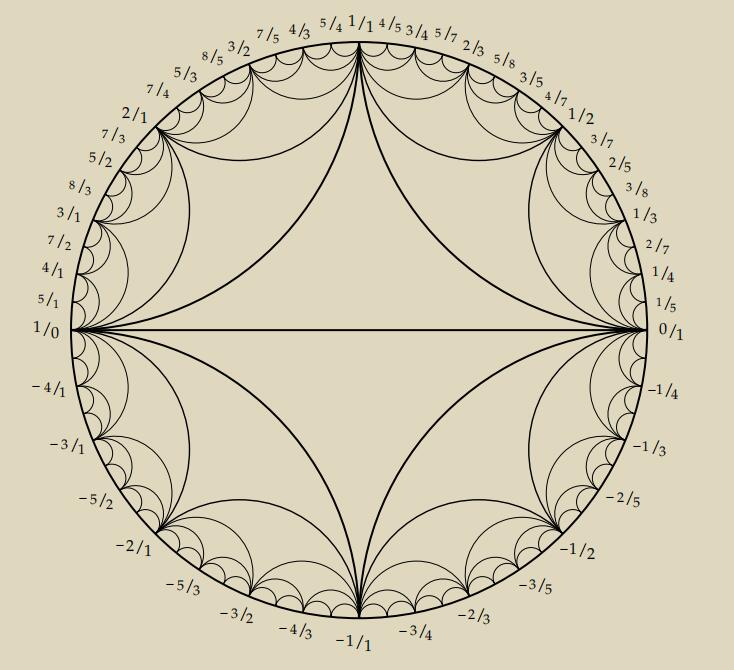
\includegraphics[scale=0.5]{FareyDiagram.jpg}
    \caption{Farey Graph}
    \label{FareyDiagram}
\end{figure}
\par
The diagram has infinitely many curvilinear triangles, getting smaller and smaller out near the boundary circle. The diagram can be constructed by first inscribing the two big
triangles in the circle, then adding the four triangles that share an edge with the two
big triangles, then the eight triangles sharing an edge with these four, then sixteen
more triangles, and so on forever. Our first task will be to explain how the vertices of all the
triangles are labeled with rational numbers.
\par
The vertices of the triangles in the Farey graph are labeled with fractions a/b,
including the fraction 1/0 for $\infty$, according to the following scheme. In the upper
half of the diagram first label the vertices of the big triangle 1/0, 0/1, and 1/1. Then one inserts labels for successively
\par
smaller triangles by the rule that, if the labels at the two ends
of the long edge of a triangle are a/b and c/d, then the label
on the third vertex of the triangle is $\frac{a+c}{b+d}$
. This fraction is called the mediant of a/b and c/d.
\par
The labels in the lower half of the diagram follow the same scheme, starting with
the labels 1/0, 0/1, and 1/1 on the large triangle. Using 1/0 instead of 1/0 as
the label of the vertex at the far left means that we are regarding $+\infty$ and $-\infty$ as the
same. The labels in the lower half of the diagram are the negatives of those in the
upper half, and the labels in the left half are the reciprocals of those in the right half.
\par
Our usual custom will be to write fractions with a positive denominator, so the
sign of the fraction is the sign of the numerator. This rule does not apply to the
ambiguous fraction $1/0 = -1/0$, of course.
\par
With a construction like this it is not easy to tell by a simple calculation whether or not two given rational numbers a/b and c/d are joined by an edge in the diagram. Fortunately there is such a criterion:
\begin{proposition}
\label{prop3.1}
For each pair of fractions $a/b$ and $c / d$, including $\pm 1 / 0$, there exists an edge in the Farey graph with endpoints labeled $a / b$ and $c / d$ if and only if the determinant $ad-bc$ of the matrix $\left(\begin{array}{ll}a&c \\ b&d\end{array}\right)$ is equal to $1$ or $-1$.
\end{proposition}
\begin{proof}
Using induction and the idea of Euclidean Algorithm we can prove it. Details are seen in \cite{hatcher2002topology}.
\end{proof}
\begin{corollary}
The mediant rule for labeling the vertices in the Farey graph always
produces labels $a / b$ that are fractions in lowest terms.
\end{corollary}
\begin{proof}
Consider an edge joining a vertex labeled $a / b$ to another vertex labeled $c / d$ From the preceding proposition we have $a d-b c=\pm 1 .$ This implies that $a$ and $b$ are coprime since any common divisor of $a$ and $b$ must divide the products ad and $b c,$ hence also the difference $a d-b c=\pm 1,$ but the only divisors of $\pm1$ are $\pm1$
\end{proof}
The preceding proposition can also be used to prove another basic fact about the
Farey graph:
\begin{proposition}
 Every fraction $a/b$ in lowest terms occurs as the label on some vertex in the Farey graph.
\end{proposition}
\begin{proof}
Still be the process of Euclidean Algorithm.
\end{proof}
Once we have the Farey graph, we can construct the \textit{Farey complex}. In our picture of the Farey graph, we can see lots of boundaries of triangles: triples of vertices that are pairwise connected by an edge. We can imagine gluing in (two-dimensional) triangles in all of those places (this can be done formally using the notion of a quotient space). The Farey complex is the space obtained by gluing in all possible triangles to the Farey graph. From the definition we saw that every edge of the Farey graph is contained in exactly two triangles.
\par
Finally, we can define the\textit{ Farey tree}. The set of vertices is the
union of the set of edges of the Farey complex and the set of triangles of the Farey
complex. We connect two vertices when there is a containment relation. In other
words, when an edge of the Farey complex is contained in a triangle of the Farey complex, we connect the corresponding vertices of the Farey tree. Because of the
way we defined the Farey tree, we can visualize it as being superimposed on the
Farey complex; see Figure \ref{FareyTree}. Just to emphasize: there are two types of vertices of the Farey tree—corresponding to edges and to triangles of the Farey complex—and
adjacent vertices have different types. 
\par
The Farey tree is indeed a tree according to our definition of Farey graph
\begin{figure}
    \centering
    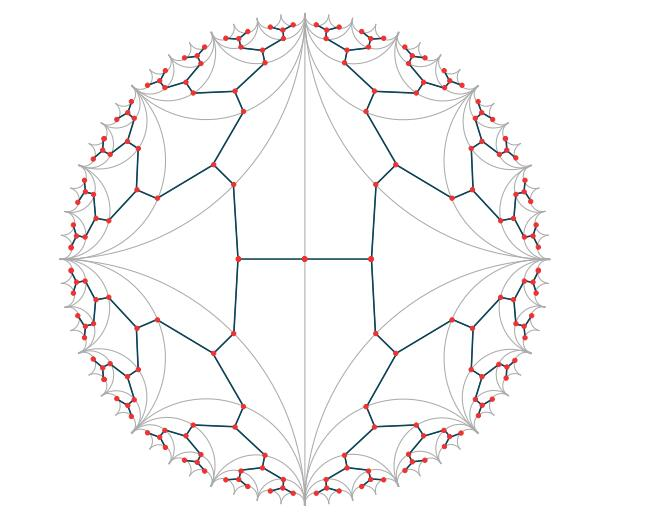
\includegraphics[scale=0.5]{FareyTree.jpg}
    \caption{The Farey tree superimposed on the Farey complex.}
    \label{FareyTree}
\end{figure}


\subsection{$SL_2(\mathbb{Z})$-action on the Farey tree}
\label{chap4.2}
For a fraction $a/b$ in lowest terms labeling on a point of the Farey Tree, we can equivalently write it as a representative $\pm(a,b)$. In this way we obtain an action of $SL_2(\mathbb{Z})$ on Farey graph by matrix multiplication (It is easy to check that the action on vertices preserves adjacency and non-adjacency  of vertices with help from proposition \ref{prop3.1}. Also, the action of $SL_2(\mathbb{Z})$ on the Farey graph induces an action on the Farey complex, meaning that the action on the graph takes the boundary of a triangle to the boundary of a triangle: Let $A\in SL_2(\mathbb{Z})$, then
$A\left(\begin{array}{lll}
p&r&p+r \\
q&s&q+s
\end{array}\right)$
preserves the graph relations of the three points $\pm(p,q),\pm(r,s),\pm(p+r,q+s)$. Again, the action of $SL_2(\mathbb{Z})$ on the Farey complex carries over to an action on the Farey tree.
\par
Now we study the properties of this action.
\\
\\
\noindent
\textit{No inversions.} Since the action of $SL_2(\mathbb{Z})$ on the Farey complex cannot interchange an edge and a triangle, the action of $SL_2(\mathbb{Z})$ on the Farey tree cannot interchange vertices of two different types. In other words, $SL_2(\mathbb{Z})$ acts on the Farey tree without inversions.
\\
\\
\noindent
\textit{Stabilizers of vertices corresponding to edges of the Farey complex.} Let us first deal with the vertex $v$ of the Farey tree corresponding to the edge of the Farey complex connecting the vertices $\pm(1,0)$ and $\pm(0,1) .$ For an element of $SL_2(\mathbb{Z})$ to stabilize
$v,$ it simply must preserve the set
\[
\{(1,0),(-1,0),(0,1),(0,-1)\}
\]
Now, the columns of a matrix are just the images of the standard basis vectors under the action of that matrix. Therefore, the columns of our stabilizer must lie in this list of four elements. That gives exactly $\left(\begin{array}{l}4 \\ 2\end{array}\right)=6$ matrices to think about. But we cannot choose a vector and its negative, for then the determinant will be 0. It turns out that the other four matrices all have determinant 1:
\[
\left(\begin{array}{ll}
1 & 0 \\
0 & 1
\end{array}\right),\left(\begin{array}{rr}
0 & 1 \\
-1 & 0
\end{array}\right),\left(\begin{array}{rr}
-1 & 0 \\
0 & -1
\end{array}\right),\left(\begin{array}{rr}
0 & -1 \\
1 & 0
\end{array}\right)
\]
These are exactly the elements of the cyclic group generated by the second matrix on the list. So the stabilizer of $v$ is a cyclic group of order 4.
\\
\\
\noindent
\textit{Stabilizers of vertices corresponding to triangles of the Farey complex. }As in the
last case, it suffices to consider the case of the vertex corresponding to the triple
\[
\pm(1,0) \quad \pm(0,1) \quad \pm(1,1)
\]
(prove the analogous claim). If an element of $SL_2(\mathbb{Z})$ fixes this vertex of the Farey tree, it must take (1,0) to one of the six vectors listed and it must take (0,1) to another one of the six vectors. But the images of these vectors are the columns of the given element of $SL_2(\mathbb{Z}),$ and so there are only a few possibilities for the stabilizer of this vertex in $SL_2(\mathbb{Z}),$ namely, the matrices
\[
\left(\begin{array}{ll}
1 & 0 \\
0 & 1
\end{array}\right),\left(\begin{array}{rr}
0 & 1 \\
-1 & 1
\end{array}\right),\left(\begin{array}{ll}
-1 & 1 \\
-1 & 0
\end{array}\right)
\]
and their negatives.
\\
\\
\noindent
\textit{Transitivity on the vertices of the Farey tree corresponding to edges of the Farey complex.} Take the vertex $v$ of the Farey tree corresponding to $\{\pm(p, q), \pm(r, s)\} .$ We will show there is an element of $SL_2(\mathbb{Z})$ taking the standard vertex $v_{0}$ given by $\{\pm(1,0), \pm(0,1)\}$ to $v .$ By the definition of the Farey tree, the determinant of
\[
\left(\begin{array}{ll}
p & r \\
q & s
\end{array}\right)
\]
is 1 (after possibly replacing $(r, s)$ with $-(r, s)$ ). But then this is the matrix we were looking for!
\\
\\
\noindent
\textit{Transitivity on the edges of the Farey tree.} Recall that an edge of the Farey tree connects one vertex corresponding to an edge of the Farey complex to one vertex corresponding to a triangle of the Farey complex. We have a favorite edge $e_{0},$ namely the one connecting the vertex $v_{0}$ corresponding to $\{\pm(1,0), \pm(0,1)\}$ to the vertex $w_{0}$ corresponding to $\{\pm(1,0), \pm(0,1), \pm(1,1)\} .$ We will show that we can take any other edge to this one using an element of $SL_2(\mathbb{Z})$.
\par
Consider an edge $e$ connecting vertices $v$ and $w$ of the Farey tree. And say that $v$ corresponds to $\{\pm(a, b), \pm(c, d)\} .$ The fact that $\pm(a, b)$ and $\pm(c, d)$ span an edge of the Farey complex means that one of the matrices
\[
A=\left(\begin{array}{ll}
a & c \\
b & d
\end{array}\right) \quad \text { or } \quad A^{\prime}=\left(\begin{array}{cc}
a & -c \\
b & -d
\end{array}\right)
\]
has determinant $1 ;$ say $A$ does. Then $A^{-1} v=v_{0} .$ We are halfway there-we just need to find a matrix $B$ that stabilizes $v_{0}$ and takes $w_{0}$ to $A^{-1} w .$ Then $B^{-1} A^{-1} e$ will be equal to $e_{0},$ as we wanted.
\par
So what is $A^{-1} w ?$ All we know is that it is some vertex of the Farey tree that is connected to $v_{0} .$ Well, there are only two of those, since an edge of the Farey complex is contained in exactly two triangles. There is $w_{0},$ and the vertex corresponding to $\{\pm(1,0), \pm(0,1), \pm(1,-1)\} ;$ call it $w_{1} .$ If $A^{-1} w=w_{0}$ there is nothing to do. But there is the possibility that $A^{-1} w=w_{1},$ and so we need to show that there is a matrix $B$ in $SL_2(\mathbb{Z})$ taking $w_{0}$ to $w_{1}$ (in other words, we are showing that the stabilizer of $v_{0}$ acts transitively on the vertices adjacent to $v_{0}$ ).
\par
Remember that we already computed the stabilizer of $v_{0}$ earlier. It is the group of matrices consisting of
\[
\left(\begin{array}{ll}
1 & 0 \\
0 & 1
\end{array}\right),\left(\begin{array}{rr}
0 & 1 \\
-1 & 0
\end{array}\right)
\]
and their negatives. But the second matrix takes the vertex $w_{0}$ to $w_{1},$ and so we have succeeded in showing that $SL_2(\mathbb{Z})$ acts transitively on the edges of the Farey tree.
\\
\\
\noindent
\textit{Stabilizers of edges} If an element of $SL_2(\mathbb{Z})$ fixes the edge $e_{0}$ we were just looking at, then it must lie in the intersection of the stabilizers of $v_{0}$ and $w_{0} .$ But this intersection is just the identity matrix and its negative.
\\
\\
After all the preparing work, we can now write down our presentation for $SL_2(\mathbb{Z})$. The hard part is already done: $SL_2(\mathbb{Z})$ acts without inversions on the Farey tree and that it acts transitively on edges, and we have already computed the stabilizers of $e_{0}, v_{0},$ and $w_{0}:$ they are isomorphic to $\mathbb{Z} / 2 \mathbb{Z}, \mathbb{Z} / 4 \mathbb{Z}$ and $\mathbb{Z} / 6 \mathbb{Z}$. Therefore, applying the theorem \ref{thm3.3}, we have the following isomorphism
\begin{theorem}
\label{thmain}
The group $SL_2(\mathbb{Z})$ can be presented as
\[
S L_{2}(\mathbb{Z}) \cong \mathbb{Z} / 4 *_{\mathbb{Z} / 2} \mathbb{Z} / 6
\]
where the subgroups $\mathbb{Z} / 2, \mathbb{Z} / 4, \mathbb{Z} / 6$ are generated by
\[
\left(\begin{array}{rr}
-1 & 0 \\
0 & -1
\end{array}\right),\left(\begin{array}{cc}
0 & 1 \\
-1 & 0
\end{array}\right),\left(\begin{array}{rr}
0 & -1 \\
1 & 1
\end{array}\right)
\]
respectively and the gluing maps $\mathbb{Z} / 2\hookrightarrow\mathbb{Z} /4$ and $\mathbb{Z} / 2\hookrightarrow\mathbb{Z} /6$ are inclusions.
\end{theorem}

\subsection{The Homology of $SL_2(\mathbb{Z})$}
Now we can calculate the homology of the linear group, $SL_2(\mathbb{Z})$.
\par
We proved the theorem \ref{thmain} in last section:
\[
S L_{2}(\mathbb{Z}) \cong \mathbb{Z} / 4 *_{\mathbb{Z} / 2} \mathbb{Z} / 6
\]
\par
Now consider the map $S L_{2}(\mathbb{Z}) \rightarrow \mathbb{Z} / 12$ defined by sending the generator of $\mathbb{Z} / 4$ to 3 mod 12 and the generator of $\mathbb{Z} / 6$ to 2 mod 12
\begin{theorem}
\label{thm3}
The $\operatorname{map} S L_{2}(\mathbb{Z}) \longrightarrow \mathbb{Z} / 12$ induces an isomorphism in integral homology:
\[
H_{i}\left(S L_{2}(\mathbb{Z}), \mathbb{Z}\right) \cong H_{i}(\mathbb{Z} / 12, \mathbb{Z}) \cong\left\{\begin{array}{ll}
\mathbb{Z} & i=0 \\
\mathbb{Z} / 12 & i \text { odd } \\
0 & i \text { even }
\end{array}\right.
\]
\end{theorem}
\begin{proof}
Associated to any decomposition $G=G_{1} *_{A} G_{2},$ there is a Mayer-Vietoris sequence as to corollary \ref{cor1}
\[
\cdots \rightarrow H_{i}(A) \rightarrow H_{i}\left(G_{1}\right) \oplus H_{i}\left(G_{2}\right) \rightarrow H_{i}(G) \rightarrow H_{i-1}(A) \rightarrow \cdots
\]
The homology of a cyclic group $\mathbb{Z} / n$ is given by example \ref{example1}
\[
H_{i}(\mathbb{Z} / n, \mathbb{Z})=\left\{\begin{array}{ll}
\mathbb{Z} & i=0 \\
\mathbb{Z} / n & i \text { odd } \\
0 & i \text { even }
\end{array}\right.
\]
Moreover, it is easy to see that if $\mathbb{Z} / n \rightarrow \mathbb{Z} /(n m)$ is the inclusion $1 \mapsto m,$ then the map $H_{2 i-1}(\mathbb{Z} / n) \rightarrow H_{2 i-1}(\mathbb{Z} /(n m))$ is the same inclusion that maps the identity 1 in the torsion part $\mathbb{Z} / n$ to m in $\mathbb{Z} / (n m)$. For example, in the following figure \ref{fig:my_label} we calculate the case $\mathbb{Z} / 2\hookrightarrow\mathbb{Z} /4$.
\begin{figure}
    \centering
    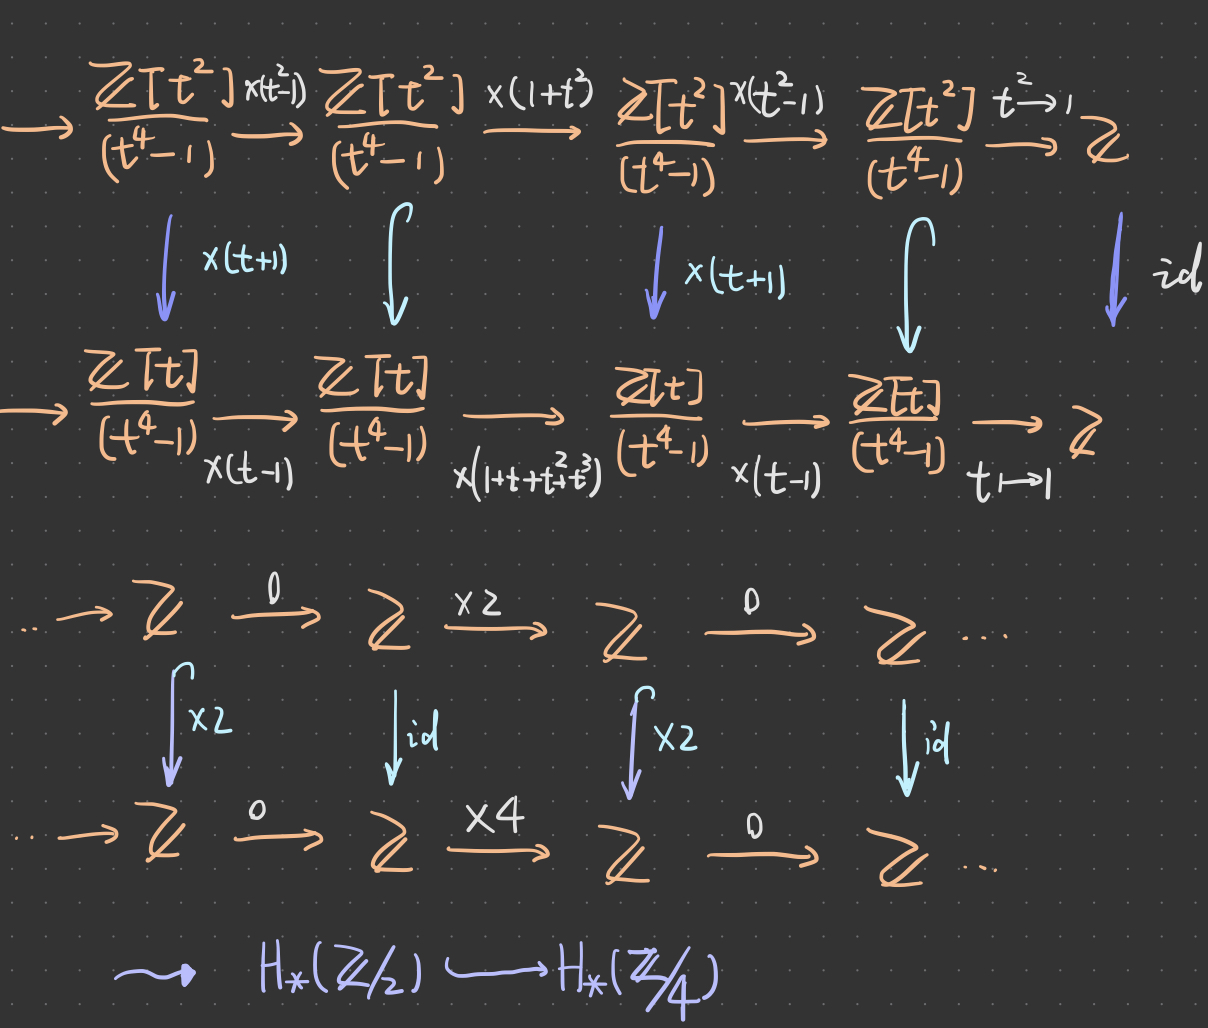
\includegraphics[scale=0.2]{injection.jpg}
    \caption{$\mathbb{Z} / 2\hookrightarrow\mathbb{Z} /4$}
    \label{fig:my_label}
\end{figure}
\newpage
It follows that the sequence for computing $H .\left(S L_{2}(\mathbb{Z})\right)$ has the following form:
\[
0 \rightarrow H_{2 i}\left(S L_{2}(\mathbb{Z})\right) \rightarrow \mathbb{Z} / 2 \rightarrow \mathbb{Z} / 4 \oplus \mathbb{Z} / 6 \rightarrow H_{2 i-1}\left(S L_{2}(\mathbb{Z})\right) \rightarrow 0
\]
$\operatorname{since} H_{2 i}(\mathbb{Z} / n)=0$ for all $n, i \geq 1 .$ Note that the $\operatorname{map} \mathbb{Z} / 2 \rightarrow \mathbb{Z} / 4 \oplus \mathbb{Z} / 6$ is
injective so that $H_{2 i}\left(S L_{2}(\mathbb{Z})\right)=0$ for $i \geq 1$ and $H_{2 i-1}\left(S L_{2}(\mathbb{Z})\right)$ has order 12 One checks easily that $H_{2 i-1}\left(S L_{2}(\mathbb{Z})\right)$ is in fact cyclic with generator $(1,2)$ .
\end{proof}

\begin{remark}
For other arithmetic linear groups, like the cohomology of $SL_2(\mathbb{Z}[1/p])$ for p prime, it was completely calculated by A. Adem and M. Naffah in \cite{adem1998cohomology}. The homology of $SL_2(\mathbb{Z}[1/m])$ for small m can be computed using a kind of algorithm introduced in \cite{bui2014homology}. For further information on the homology of $SL_2(R)$ for R being one dimensional ring, one can refer to Chapter.4 of \cite{knudson2012homology} and its Chapter.5 for further application of these results.
\end{remark}

